\chapter{Metodologia específica: controle do sistema hidráulico não linear}
\label{cap:controle}

Este capítulo apresenta a metodologia adotada para o projeto e a avaliação, em simulação, de uma estratégia de controle digital de pressão de freio que utiliza o módulo hidráulico de uma unidade ABS/ESC como atuador de pressão do freio de serviço. O estudo é desenvolvido em ambiente simulado, com possibilidade de extensão para ensaios em bancada, considerando um canal/roda (modelo concentrado em duas pressões) e implementação digital em tempo discreto, com faixas de pressão compatíveis com a aplicação e período de amostragem compatível com ECUs automotivas.

O foco é o seguimento de uma referência de pressão por roda, obtida a partir de um controlador longitudinal de nível superior (por exemplo, um ACC), e a avaliação do compromisso entre desempenho dinâmico e esforço de atuação imposto pelas limitações físicas do módulo hidráulico.

O problema de pesquisa é formulado da seguinte maneira: como projetar e implementar um controlador digital em espaço de estados que permita ao módulo hidráulico ABS/ESC rastrear perfis de pressão $P_{\mathrm{ref}}(t)$ por roda, garantindo desempenho dinâmico adequado e esforço de atuação compatível com as limitações físicas do sistema?

A hipótese considerada é que um controlador LQ em tempo discreto (LQI) com observador de Luenberger, sintetizado a partir da linearização local de um modelo não linear em duas pressões, é capaz de rastrear referências de pressão por roda com erro estacionário nulo e dinâmica satisfatória, desde que: (i) o ponto de operação satisfaça $\Delta P>0$ nas válvulas, (ii) as saturações sejam parametrizadas de forma fisicamente consistente e (iii) o período de amostragem seja compatível com a banda do atuador.

O objetivo geral é demonstrar, em simulação, que o módulo hidráulico ABS/ESC pode atuar como atuador principal de pressão do freio de serviço, acompanhando $P_{\mathrm{ref}}(t)$ derivado de requisitos de desaceleração.

Os objetivos específicos são:
\begin{enumerate}
    \item Modelar o subsistema hidráulico por um modelo não linear em duas pressões ($P_{sup},P_w$) e realizar uma validação qualitativa em malha aberta.
    \item Linearizar o modelo em torno de um ponto de operação $(x_0,u_0)$ fisicamente consistente, obtendo as matrizes $(A,B,C,D)$.
    \item Discretizar o sistema e projetar um controlador LQI discreto, com observador de Luenberger, para regular a velocidade da bomba ($\omega_p$), em conjunto com uma lógica discreta (on/off com histerese) para as válvulas de entrada e saída.
    \item Avaliar o seguimento de $P_{\mathrm{ref}}(t)$ e o esforço de controle sob saturações físicas de pressão e dos atuadores.
\end{enumerate}

O capítulo está organizado da seguinte forma: inicialmente descreve-se o mapeamento de desaceleração para referência de pressão (Seção~\ref{sec:mapeamento-aref-pressao}) e o modelo hidráulico não linear 2P (Seção~\ref{sec:controle-4-1}); em seguida, apresenta-se a linearização e a formulação em espaço de estados (Seções~\ref{sec:controle-linearizacao-2p} e \ref{sec:controle-formulacao-espaço-estados}); por fim, descrevem-se a síntese do controlador/observador, a discretização e a implementação em Simulink (Seções~\ref{sec:controle-lqr-luenberger} a \ref{sec:implementacao-simulink}). Os procedimentos de simulação e as métricas adotadas são resumidos na Seção~\ref{sec:procedimentos-simulacao-controle}, e os resultados são apresentados e discutidos no Capítulo~\ref{chap:resultados}.


%====================================================================
%====================================================================
%====================================================================
%====================================================================
\section{Da desaceleração à referência de pressão por roda}
\label{sec:mapeamento-aref-pressao}
Admite-se que um controlador longitudinal de nível superior fornece a desaceleração desejada $a_{\mathrm{ego}}(t)$. Para converter esse requisito em uma referência de pressão por roda, adota-se um mapeamento quase estático baseado na cadeia
\emph{desaceleração $\rightarrow$ força longitudinal $\rightarrow$ torque de frenagem $\rightarrow$ pressão hidráulica}.

As hipóteses simplificadoras são: (i) a dinâmica longitudinal de alto nível é lenta quando comparada ao controle de pressão; (ii) o deslizamento longitudinal da roda não é explicitamente modelado neste mapeamento (isto é, a conversão força--torque utiliza raio efetivo $R_w$); (iii) efeitos como transferência de carga, variação do coeficiente de atrito pneu--solo e conformidade mecânica são agregados em ganhos efetivos.

Define-se inicialmente a força longitudinal de frenagem desejada no canal/roda modelado como
\begin{equation}
    F_{x,w}^{\mathrm{des}}(t) = \kappa_w\, m\,\big|a_{\mathrm{ego}}(t)\big|,
    \label{eq:mapeamento_aref_forca}
\end{equation}
em que $m$ é a massa do veículo e $\kappa_w\in(0,1]$ representa um fator de repartição (por eixo e por roda). Em alternativa, pode-se empregar uma massa equivalente por roda $m_{\mathrm{eq}}$ e tomar $\kappa_w=1$.

O torque de frenagem desejado no cubo é então aproximado por
\begin{equation}
    T_{b,w}^{\mathrm{des}}(t) = R_w\,F_{x,w}^{\mathrm{des}}(t).
    \label{eq:mapeamento_aref_torque}
\end{equation}

Por fim, relaciona-se o torque de frenagem à pressão hidráulica no cáliper por um ganho agregado (quase estático) $K_{br}$:
\begin{equation}
    T_{b,w}(t) \approx K_{br}\,P_w(t)
    \qquad\Rightarrow\qquad
    P_{\mathrm{ref}}(t) = \frac{T_{b,w}^{\mathrm{des}}(t)}{K_{br}}.
    \label{eq:mapeamento_aref_pressao}
\end{equation}

Uma forma equivalente é explicitar $K_{br}$ a partir da geometria do conjunto de freio, por exemplo, assumindo $T_{b,w}\propto \mu_p\,F_{cl}\,R_{eff}$ e $F_{cl}=P_w\,A_{cal}$, o que agrega (em $K_{br}$) o coeficiente de atrito pastilha--disco $\mu_p$, o raio efetivo do disco $R_{eff}$, a área efetiva do cáliper $A_{cal}$ e fatores geométricos do atuador. Nas simulações realizadas, $P_{\mathrm{ref}}(t)$ é sempre especificada por roda e tratado como sinal externo ao regulador de pressão.

%====================================================================
%====================================================================
%====================================================================
%====================================================================
\section{Modelo hidráulico não linear de duas pressões}
\label{sec:controle-4-1}
A planta controlada é o módulo hidráulico da unidade ABS/ESC, empregado como atuador de pressão do freio de serviço. A literatura indica a utilidade de modelos concentrados para descrever a relação entre comandos de válvulas, pressão no cilindro da roda e força de frenagem, tanto para projeto de controladores quanto para validação \emph{hardware-in-the-loop} \cite{HouhuaJing2022,PressureCoordinatedControl2023,ZengYangHuang2023,MotorParametricDesign2023}.

Neste trabalho, adota-se um modelo em duas pressões, $P_{sup}$ (suprimento/manifold) e $P_w$ (canal/roda), em linha com \citeonline{HouhuaJing2022,ZengYangHuang2023,Lv2014}.

Para fins de projeto, definem-se os vetores de estado e comando como:
\begin{equation}
    x(t) =
    \begin{bmatrix}
        P_{sup}(t) \\[2pt]
        P_{w}(t)
    \end{bmatrix},
    \qquad
    u(t) =
    \begin{bmatrix}
        \omega_p(t) \\[2pt]
        u_{in}(t)   \\[2pt]
        u_{out}(t)
    \end{bmatrix}.
    \label{eq:vect-estados-hidraulico}
\end{equation}


%====================================================================
%====================================================================
%====================================================================
%====================================================================
\subsection{Estratégias de acionamento das válvulas}
\label{sec:controle-4-1-1}

O módulo hidráulico é composto por uma bomba de deslocamento variável, válvulas de entrada (pressurização) e de saída (alívio) para cada canal/roda, e um suprimento de fluido. As válvulas podem ser do tipo on/off (solenóides) ou proporcionais (HSV/USV), o que abre diferentes possibilidades de estratégia de acionamento.

Na literatura, destacam-se duas abordagens usuais:
\begin{itemize}
    \item \textbf{Modulação quase linear de queda de pressão}: válvulas on/off operam em torno de um ponto de equilíbrio no qual a queda de pressão varia aproximadamente de forma linear com a corrente/condutância, permitindo o uso de relações vazão–comando simplificadas para projeto \cite{ChenLv2017}.
    \item \textbf{PWM em válvulas HSV/USV}: o ciclo de trabalho governa a taxa de pressurização/alívio, solução compatível com arquiteturas embarcadas e eficaz para rastreamento dinâmico de pressão \cite{HouhuaJing2022}.
\end{itemize}

Neste trabalho, o modelo matemático adota válvulas on/off e $u_{in}$ e $u_{out}$ são tratados como comandos discretos (aberto/fechado). Para evitar comutações excessivas na presença de ruído e discretização, emprega-se uma histerese sobre o erro de seguimento $e(t)=P_{w,\text{ref}}(t)-P_w(t)$ na geração desses sinais. Em uma implementação embarcada, é possível ainda interpretar $u_{in}$ e $u_{out}$ como sinais de modulação PWM (ciclo de trabalho) e adotar um modelo médio; no presente estudo, prioriza-se a lógica on/off para representar o comportamento típico de válvulas solenóides.

%====================================================================
%====================================================================
%====================================================================
%====================================================================
\subsection{Dinâmica e leis de vazão}
\label{sec:controle-modelo-hidraulico-2p}

Adota-se uma representação \emph{lumped-parameter} com duas regiões compressíveis: (i) suprimento, $P_{sup}$, volume $V_{sup}$ e retorno $P_{ret}$; (ii) canal de roda, $P_w$, volume $V_w$.

A partir da equação de continuidade para fluido compressível, obtém-se:

\begin{equation}
    \dot{P}_{sup} = \frac{\beta}{V_{sup}}\Big(Q_{pump} - Q_{in} - Q_{\text{leak},sup}\Big),
    \quad
    \dot{P}_{w} = \frac{\beta}{V_{w}}\Big(Q_{in} - Q_{out} - Q_{\text{leak},w}\Big),
    \label{eq:din_press}
\end{equation}

em que $\beta$ é o módulo volumétrico efetivo e as vazões são modeladas a seguir.

A vazão da bomba hidráulica é descrita por
\begin{equation}
    Q_{pump} = K_b\,\omega_p - K_{lb}\big(P_{sup}-P_{ret}\big),
    \label{eq:qpump_2p}
\end{equation}
em que $K_b$ agrega deslocamento e eficiência volumétrica, e $K_{lb}$ representa o vazamento interno para o retorno \cite{MotorParametricDesign2023,WangBingbing2015}.

As válvulas de entrada e de saída são modeladas por uma lei de orifício, derivada da equação de Bernoulli (forma de Torricelli) e corrigida por um coeficiente de descarga $C_d$:

\begin{equation}
    Q = C_d\,A_{ef}\,\sqrt{\frac{2\,\Delta P}{\rho}},
    \label{eq:lei-orificio}
\end{equation}

\begin{equation}
    Q_{in} = C_{d,in}\,A_{in}(u_{in})\sqrt{\frac{2\,\big(P_{sup}-P_w\big)_{+}}{\rho}},
    \qquad
    Q_{out} = C_{d,out}\,A_{out}(u_{out})\sqrt{\frac{2\,\big(P_{w}-P_{ret}\big)_{+}}{\rho}},
    \label{eq:qin_qout}
\end{equation}
em que $(\cdot)_{+}=\max(\cdot,0)$.

Adota-se $A_{in}(u_{in}) = A_{in,\max}\,u_{in}$, $A_{out}(u_{out}) = A_{out,\max}\,u_{out}$ e $u_{in},u_{out}\in[0,1]$ \cite{ProportionalPressureABS2023,Lv2014,ChenLv2017}.

Os vazamentos internos no suprimento e no canal de roda são representados por termos proporcionais à diferença de pressão em relação ao retorno:
\begin{equation}
    Q_{\text{leak},sup} = K_{ls},\big(P_{sup}-P_{ret}\big),
    \qquad
    Q_{\text{leak},w} = K_{lw},\big(P_{w}-P_{ret}\big).
    \label{eq:leaks}
\end{equation}














%====================================================================
%====================================================================
%====================================================================
%====================================================================
\subsection{Simulação em malha aberta e validação do modelo hidráulico}
\label{sec:controle-validacao-2p}
Esta subseção descreve o ensaio em malha aberta utilizado para verificar, de forma qualitativa, a causalidade do modelo e a coerência física dos transientes de pressurização, retenção e alívio, antes da inserção do controlador.

O ensaio em malha aberta é organizado por meio de um \textit{script} MATLAB associado ao modelo em Simulink. Esse \textit{script} define o horizonte de simulação e o período de amostragem, configura os parâmetros do modelo hidráulico (volumes equivalentes, coeficientes de vazão e saturações) e gera os sinais de comando da bomba e das válvulas para as três fases do ensaio (pressurização, retenção e alívio), de modo a reproduzir cenários típicos descritos na literatura \cite{ZengYangHuang2023,Lv2014,HouhuaJing2022}. Ao final de cada simulação, são registrados os perfis de pressão no suprimento e no canal de roda, bem como as vazões e os comandos de válvula, que são utilizados para visualização gráfica e cálculo de indicadores. A arquitetura geral da simulação, incluindo o modelo hidráulico, os sinais de comando $(\omega_p,u_{in},u_{out})$ e os blocos de registro de dados, é ilustrada nas Figuras~\ref{fig:bloco_matlab_function_2p} e \ref{fig:simulink_ensaio_2p}. O código completo (bloco hidráulico 2P e \textit{script} do ensaio) encontra-se no Apêndice~\ref{ap:scripts-matlab} (Códigos~\ref{cod:bloco_hidraulico_2p} e \ref{cod:ensaio_integrado_malha_aberta}).

\begin{figure}[htbp]
    \centering
    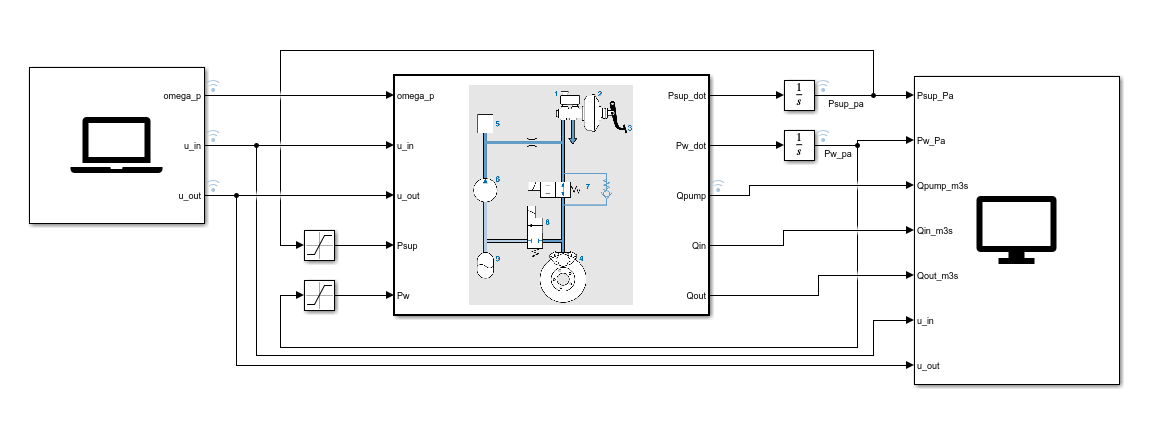
\includegraphics[width=0.90\textwidth]{figuras/image_matlab_function_bloco_hidraulico_2p.png}
    \Caption{\label{fig:bloco_matlab_function_2p} Implementação do subsistema hidráulico em um bloco \texttt{MATLAB Function} no Simulink.}
\end{figure}

\begin{figure}[htbp]
    \centering
    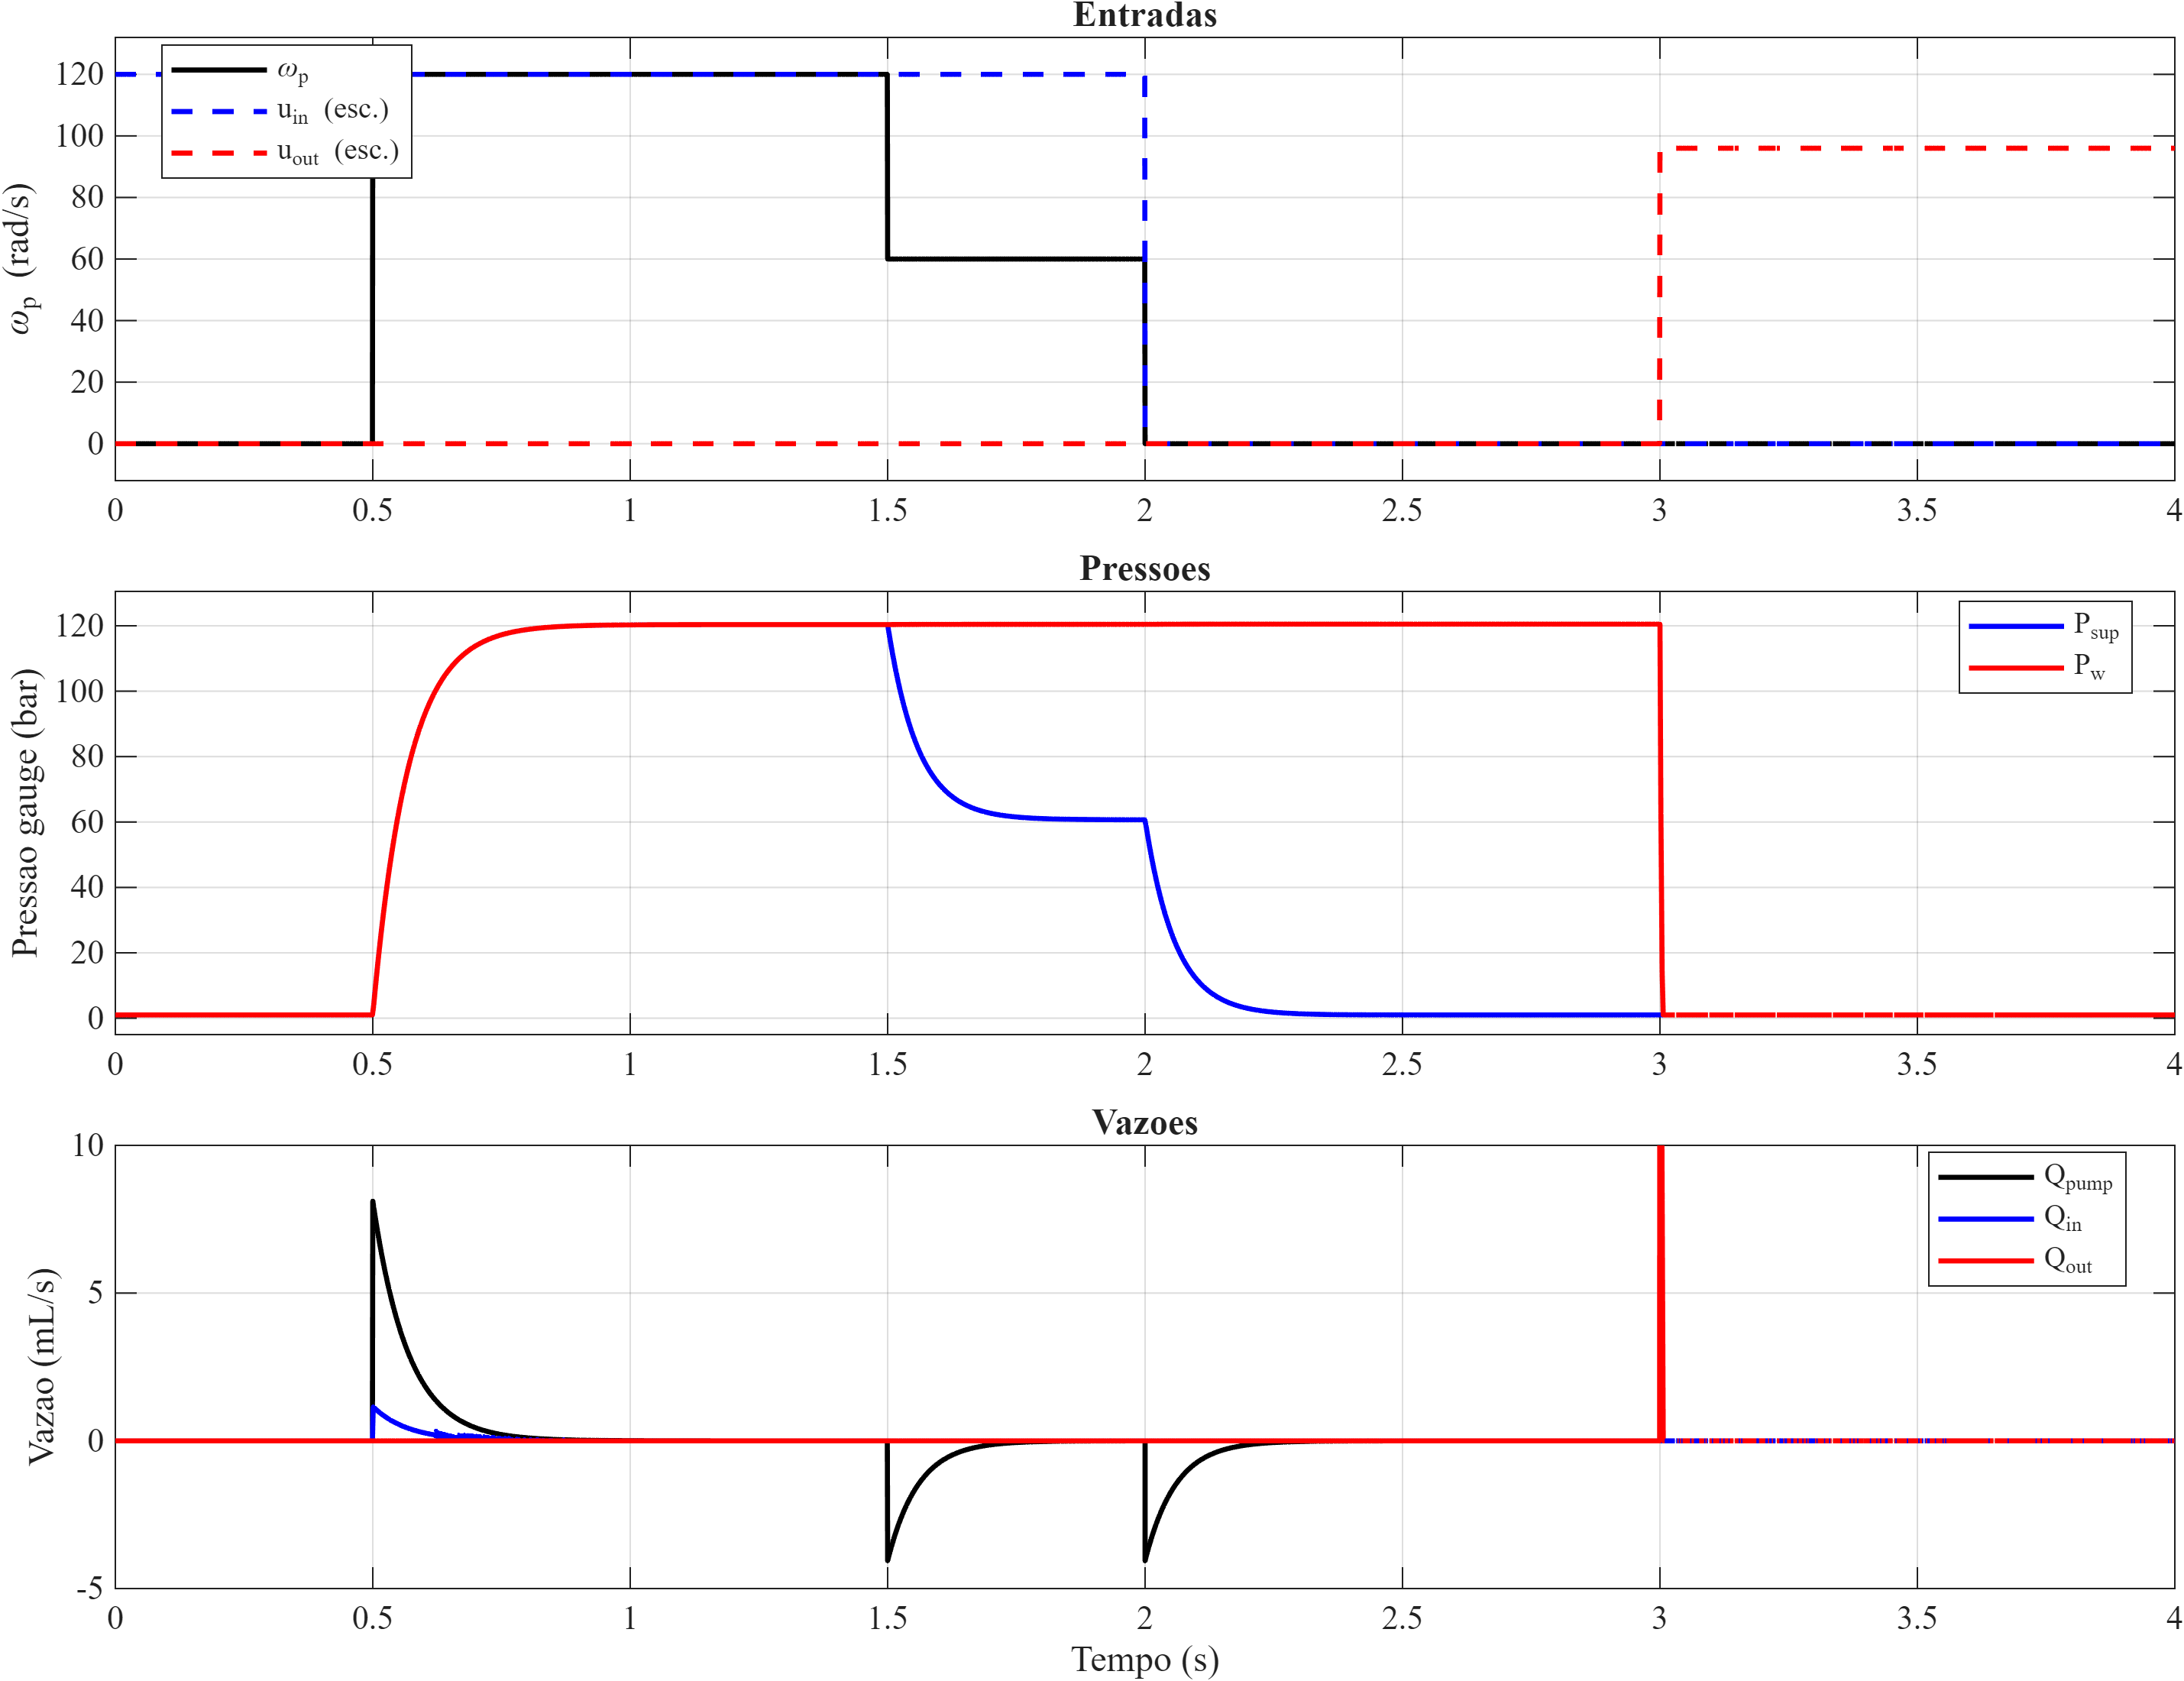
\includegraphics[width=0.85\textwidth]{figuras/ensaio_malha_aberta_integrado.png}
    \Caption{\label{fig:simulink_ensaio_2p} Esquema da simulação em malha aberta do modelo hidráulico 2P em MATLAB/Simulink, com \textit{script} MATLAB gerando o ensaio.}
\end{figure}

O ensaio em malha aberta é organizado em três fases consecutivas: (A) \textit{pressurização}, com degrau em $\omega_p$, $u_{in}=1$ e $u_{out}=0$; (B) \textit{retenção}, com $\omega_p=0$ e $u_{in}=u_{out}=0$; e (C) \textit{alívio}, com $\omega_p=0$, $u_{in}=0$ e degrau em $u_{out}$. As pressões são reportadas como \emph{gauge} em bar,
\begin{equation}
    P_{g}(t) = \frac{P(t)-P_{ret}}{10^5}\ \text{[bar]},
    \label{eq:pressao_gauge_bar_reescrita}
\end{equation}
o que permite comparar diretamente as curvas simuladas com faixas típicas de operação de unidades ESC/ABS.

Para aproximar o modelo das ordens de grandeza observadas em unidades comerciais (8--13 MPa no suprimento e variações rápidas de $P_w$) \cite{ZengYangHuang2023,HouhuaJing2022}, adotou-se um conjunto de parâmetros considerado “realista”, reduzindo $V_{sup}$ e $V_w$ e aumentando a capacidade da bomba. A Tabela~\ref{tab:parametros_hidraulico_realista_reescrita} resume os principais valores utilizados.

\begin{table}[htbp]
    \Caption{\label{tab:parametros_hidraulico_realista_reescrita} Parâmetros ajustados para faixa de pressão realista do modelo 2P}
    \UNIFORtab{}{
        \begin{tabular}{ l | l | l | l }
            \hline
            Parâmetro                          & Símbolo        & Valor adotado           & Unidade      \\
            \hline
            Densidade do fluido                & $\rho$         & 850                     & kg/m$^3$     \\
            Módulo volumétrico efetivo         & $\beta$        & $1{,}5 \times 10^9$     & Pa           \\
            Pressão de retorno                 & $P_{ret}$      & $1{,}0 \times 10^5$     & Pa           \\
            Volume equivalente do suprimento   & $V_{sup}$      & $6{,}0 \times 10^{-5}$  & m$^3$        \\
            Volume equivalente do canal/roda   & $V_{w}$        & $1{,}0 \times 10^{-5}$  & m$^3$        \\
            Coeficiente de descarga (orifício) & $C_d$          & 0{,}62                  & ---          \\
            Área máx. da válvula de entrada    & $A_{in,\max}$  & $3{,}0 \times 10^{-7}$  & m$^2$        \\
            Área máx. da válvula de saída      & $A_{out,\max}$ & $3{,}0 \times 10^{-7}$  & m$^2$        \\
            Vazamento interno da bomba         & $K_{lb}$       & $1{,}0 \times 10^{-11}$ & (m$^3$/s)/Pa \\
            \hline
        \end{tabular}
    }{\Fonte{Com base em \cite{ZengYangHuang2023,ProportionalPressureABS2023,Lv2014,ChenLv2017}.}}
\end{table}

A validação em malha aberta é realizada em duas etapas: em um \emph{caso base}, inspecionam-se causalidade, sinais de vazão e efeito das saturações, verificando se o comportamento qualitativo é coerente com a física de pressurização, retenção e alívio; em seguida, em um \emph{caso realista}, os volumes e os parâmetros da bomba são ajustados segundo a Tabela~\ref{tab:parametros_hidraulico_realista_reescrita}, de modo a reproduzir ordens de grandeza de pressão e vazão reportadas na literatura. Os resultados e a discussão desses ensaios são apresentados no Capítulo~\ref{chap:resultados}.



















%====================================================================
%====================================================================
%====================================================================
%====================================================================
\section{Linearização do modelo não linear}
\label{sec:controle-linearizacao-2p}



\subsection{Definição do ponto de operação}
\label{sec:definicao-ponto-operacao}
Adota-se um ponto de operação $(x_0,u_0)$ correspondente a regime de frenagem, com $P_{sup,0}>P_{w,0}>P_{ret}$ e $\Delta P>0$ nas leis de orifício. Para a obtenção de um modelo linear de projeto com uma única entrada, assume-se ainda $u_{in}=u_{in,0}$ constante e $u_{out}=0$ (válvula de saída fechada) no ponto de operação, de modo que a dinâmica incremental seja governada pela variável contínua $\omega_p$. O ponto de operação é escolhido de modo a representar equilíbrio local (regime permanente), isto é, $\dot{x}=f(x,u)=0$ em $(x_0,u_0)$ para as hipóteses adotadas. Os valores numéricos empregados nas simulações são apresentados no Apêndice~\ref{ap:ponto-operacao}.
\subsection{Jacobianos e forma linear aproximada}
\label{sec:derivacao-matrizes-jacobianas}
A partir de \eqref{eq:din_press}–\eqref{eq:leaks}, escreve-se $\dot{x}=f(x,u)$. As jacobianas
\[
    A=\left.\frac{\partial f}{\partial x}\right|_{x_0,u_0},
    \qquad
    B=\left.\frac{\partial f}{\partial u}\right|_{x_0,u_0}
\]
são obtidas impondo $\Delta P>0$ no ponto de operação. A linearização de primeira ordem em torno de $(x_0,u_0)$ fornece, em variáveis incrementais $\delta x = x-x_0$ e $\delta u = u-u_0$, a aproximação local
\[
    \delta\dot{x} = A\,\delta x + B\,\delta u.
\]
Como o modelo de projeto considera $u=\omega_p$ (com $u_{in}$ fixado no ponto e $u_{out}=0$), $B\in\mathbb{R}^{2\times 1}$ é uma matriz-coluna. Dessa forma, $A$ e $B$ são matrizes reais. Reportam-se apenas os autovalores de $A$ (localizados no semiplano esquerdo), indicando estabilidade local. As matrizes numéricas completas são apresentadas no Apêndice~\ref{ap:matrizes-lin}.
\subsection{Não linearidades e região de validade}
A lei de orifício implica ganho incremental $\partial Q/\partial \Delta P \propto 1/\sqrt{\Delta P}$, de modo que o ganho efetivo do sistema varia com o ponto de operação. A linearização (expansão de Taylor de primeira ordem) é, portanto, uma aproximação local; desvios significativos em relação ao ponto escolhido podem alterar margens de estabilidade e desempenho. A validação em malha fechada é conduzida sobre um perfil de referência definido em patamares e é apresentada no Capítulo~\ref{chap:resultados}, com sumarização por métricas usuais de desempenho.
%====================================================================
\section{Formulação em espaço de estados}
\label{sec:controle-formulacao-espaço-estados}
A representação linearizada empregada para síntese do controlador é dada por
\[
    \delta\dot{x} = A\,\delta x + B\,\delta u, \qquad \delta y = C\,\delta x,
\]
em que $\delta x = x-x_0$, $\delta u = u-u_0$ e $\delta y = y-y_0$, com $x=[P_{sup}\ \ P_w]^\top$, $u=\omega_p$ e $y=P_w$. Nesta formulação, as válvulas são tratadas como elementos de comutação no modelo não linear (Seção~\ref{sec:implementacao-simulink}): $u_{in}$ e $u_{out}$ são gerados por uma lógica discreta com histerese, enquanto o controlador LQI regula $\omega_p$ para atender aos requisitos de seguimento de $P_{w,\text{ref}}(t)$.
%====================================================================
\section{Projeto do controlador discreto (LQI) para a bomba hidráulica}
\label{sec:controle-lqr-luenberger}
O controlador é sintetizado em tempo discreto, a partir das matrizes $(A_d,B_d,C_d)$ obtidas por discretização ZOH do modelo linearizado com entrada $u=\omega_p$. O ponto de partida é o LQR discreto (\texttt{dlqr}), e em seguida adiciona-se ação integral para eliminação de erro estacionário, resultando em um LQI.
%--------------------------------------------------------------------
\section{Projeto do observador de Luenberger}
\label{sec:projeto-observador-luenberger}
Para estimação de estados, utiliza-se um observador de Luenberger:
\[
    \dot{\hat{x}} = A\,\hat{x} + B_c\,u_c + L\,(y-\hat{y}),
    \qquad \hat{y}=C\,\hat{x}.
\]
Definindo o erro $e=x-\hat{x}$, obtém-se $\dot{e}=(A-LC)e$. O ganho $L$ é calculado por alocação de polos (\texttt{place} em $(A^\top,C^\top)$), de forma que os polos do observador sejam mais rápidos do que os da malha fechada do controlador.

Na implementação discreta, utiliza-se a forma equivalente
\[
    \hat{x}(k+1)=A_d\,\hat{x}(k)+B_d\,u(k)+L_d\,\big(y(k)-\hat{y}(k)\big),\qquad \hat{y}(k)=C_d\,\hat{x}(k),
\]
em que $L_d$ é obtido por alocação de polos no domínio discreto, de modo a tornar a dinâmica de estimação mais rápida do que a dinâmica de controle.
%====================================================================
\section{Discretização do sistema}
\label{sec:discretizacao-sistema}
\subsection{Modelo discreto}
\label{sec:modelo-discreto}
A discretização por retenção de ordem zero (ZOH), com período de amostragem $T_s$, resulta em
\[
    x(k+1)=A_d\,x(k)+B_d\,u(k),\qquad y(k)=C_d\,x(k),
\]
com $T_s=10^{-4}$~s no presente estudo. As matrizes discretas são obtidas por \texttt{c2d}.
\subsection{LQR discreto}
\label{sec:projeto-lqr-discreto}
No domínio discreto, o LQR minimiza
\[
    J=\sum_{k=0}^{\infty} \big(x^\top Q\,x + u^\top R\,u\big),
\]
fornecendo a lei $u(k)=-K_d x(k)$ via \texttt{dlqr(A\_d,B\_d,Q,R)}. Para seguimento de referência, é adicionada ação integral, resultando em um controlador LQI.
%====================================================================
\section{Projeto do controlador LQI discreto}
\label{sec:controle-lqi-discreto}
\subsection{Sistema aumentado com ação integral}
\label{sec:lqi-mimo}
Para $x\in\mathbb{R}^2$, $u=\omega_p\in\mathbb{R}$ e $y=P_w$, define-se o integrador do erro:
\[
    z(k+1)=z(k)+T_s\big(r(k)-y(k)\big).
\]
O sistema aumentado é dado por
\[
    x_{aug}(k+1)=
    \underbrace{\begin{bmatrix}
            A_d      & 0 \\
            -C_d T_s & 1
        \end{bmatrix}}_{A_a}
    x_{aug}(k)
    +
    \underbrace{\begin{bmatrix}
            B_d \\
            0
        \end{bmatrix}}_{B_a}
    u(k)
    +
    \begin{bmatrix}
        0_{2\times 1} \\
        T_s
    \end{bmatrix}r(k),
\]
com $x_{aug}=[x^\top\ \ z]^\top\in\mathbb{R}^3$ e $B_a\in\mathbb{R}^{3\times 1}$. A lei LQI assume a forma
\[
    u(k)=-K_x\,x(k)-K_i\,z(k).
\]
em que $K_x\in\mathbb{R}^{1\times 2}$ e $K_i\in\mathbb{R}$ são obtidos a partir da solução da equação de Riccati discreta:
\[
    J=\sum_{k=0}^{\infty}\big(x_{aug}^\top Q_a x_{aug}+u^\top R\,u\big),\qquad
    Q_a\succeq 0,\ R\succ 0.
\]
\subsection{Escolha de pesos e saturações}
Um exemplo de pesos é
\[
    Q_a=\mathrm{diag}(10^{-12},\ 10^{-10},\ 10^{4}),\qquad
    R=r_{\omega}.
\]
O integrador recebe peso elevado para garantir eliminação de erro de regime ($e_\infty$), enquanto os pesos dos estados evitam problemas de escalonamento decorrentes das magnitudes de pressão em Pa. A parametrização das saturações deve ser física; limites artificiais podem induzir \emph{windup}. A partir dos ensaios apresentados no Capítulo~\ref{chap:resultados}, verifica-se que limites coerentes (pressões máximas, saturação de $\omega_p$ e histerese na lógica das válvulas) permitem o seguimento do perfil de referência sem operação permanentemente saturada.
A dinâmica em malha fechada do sistema aumentado é
\[
    x_{aug}(k+1)=
    \begin{bmatrix}
        A_d - B_d K_x & - B_d K_i \\
        -C_d T_s      & 1
    \end{bmatrix}
    x_{aug}(k),
\]
cujas raízes devem estar estritamente dentro do círculo unitário.

%====================================================================
\section{Implementação no modelo não linear em Simulink}
\label{sec:implementacao-simulink}
\subsection{Estrutura do controlador}
\label{sec:estrutura-controlador-simulink}
O modelo é executado em passo fixo com $T_s=10^{-4}$~s. A referência $P_{w,\text{ref}}(t)$ é alimentada por meio de um bloco \texttt{timeseries}. Os ganhos $K_x$, $K_i$ e $L_d$ são carregados do \texttt{workspace}. A arquitetura emprega o observador de Luenberger discreto, a lei LQI e blocos de saturação ajustados às limitações do sistema (pressões e atuadores). A execução dos ensaios em Simulink é automatizada por \textit{scripts} MATLAB que centralizam: (i) a síntese dos ganhos, (ii) a definição do perfil de referência, (iii) a parametrização do modelo e (iv) o registro dos sinais de interesse para cálculo de métricas. O \textit{script} completo utilizado para sintetizar os ganhos e executar o modelo Simulink é apresentado no Apêndice~\ref{ap:scripts-matlab} (Código~\ref{cod:script_controle_lqi_luenberger}). O código do bloco \texttt{MATLAB Function} do controlador (LQI + observador) e a lógica discreta de válvulas são fornecidos no mesmo apêndice (Códigos~\ref{cod:matlab_function_lqi_observer} e \ref{cod:matlab_function_valvulas_onoff}).

\begin{figure}[htbp]
    \centering
    \IfFileExists{figuras/simulink_freio_lqi_integrado.png}{%
        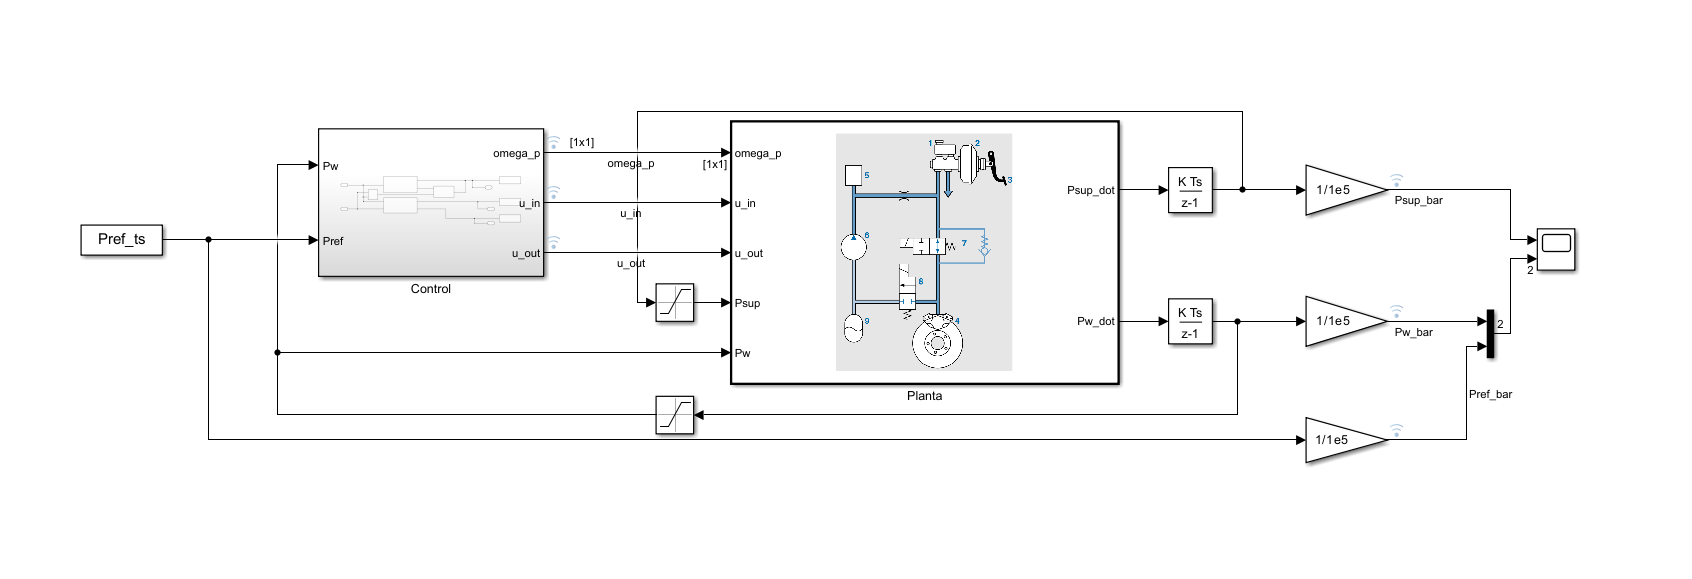
\includegraphics[width=0.92\textwidth]{figuras/simulink_freio_lqi_integrado.png}%
    }{%
        \fbox{\parbox{0.92\textwidth}{\centering\vspace{8mm}
                \textbf{Figura pendente:} salvar a captura do modelo Simulink integrado como\\
                \texttt{figuras/simulink\_freio\_lqi\_integrado.png}.\vspace{8mm}}}%
    }
    \Caption{\label{fig:simulink_freio_lqi_integrado} Modelo Simulink integrado para validação do controle digital de pressão (referência, controlador LQI+observador, lógica das válvulas e planta não linear).}
\end{figure}

\begin{figure}[htbp]
    \centering
    \IfFileExists{figuras/image_matlab_function_lqi_observer.png}{%
        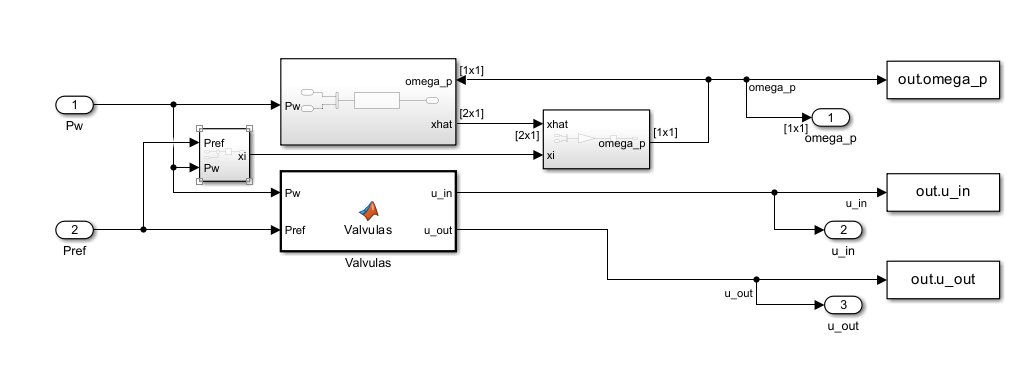
\includegraphics[width=0.85\textwidth]{figuras/image_matlab_function_lqi_observer.png}%
    }{%
        \fbox{\parbox{0.85\textwidth}{\centering\vspace{8mm}
                \textbf{Figura pendente:} salvar a captura do bloco \texttt{MATLAB Function} do controlador como\\
                \texttt{figuras/image\_matlab\_function\_lqi\_observer.png}.\vspace{8mm}}}%
    }
    \Caption{\label{fig:bloco_matlab_function_lqi_observer} Implementação do controlador discreto (LQI + observador de Luenberger) em um bloco \texttt{MATLAB Function} no Simulink.}
\end{figure}
\subsection{Integração com a planta hidráulica}
\label{sec:integracao-planta-hidraulica}
A planta não linear, descrita por \eqref{eq:din_press}–\eqref{eq:leaks}, é implementada em um bloco \texttt{MATLAB Function}. São impostas as restrições $\omega_p\ge 0$, $u_{in},u_{out}\in[0,1]$ e $P\ge P_{ret}$. Esse arranjo permite avaliar a robustez do LQI frente às não linearidades associadas a $\sqrt{\Delta P}$, à compressibilidade do fluido e às limitações físicas do atuador.
%====================================================================
\section{Procedimentos de simulação e métricas de avaliação}
\label{sec:procedimentos-simulacao-controle}
Os ensaios numéricos são conduzidos no ambiente MATLAB/Simulink de forma reprodutível, com \textit{scripts} responsáveis por configurar o modelo, executar as simulações e registrar os sinais necessários à avaliação. A intenção, no texto principal, é explicitar \emph{o papel} desses \textit{scripts} (organização do ensaio e rastreabilidade dos resultados), deixando detalhes de implementação para o Apêndice~\ref{ap:scripts-matlab}.

Na validação em malha fechada, o perfil de referência $P_{w,\text{ref}}(t)$ é definido em patamares (em bar, posteriormente convertidos para Pa): $0\rightarrow 50\rightarrow 30\rightarrow 80\rightarrow 20\rightarrow 100$. Para cada simulação, são registrados os sinais de pressão ($P_{sup}$ e $P_w$), as vazões (quando aplicável) e os comandos dos atuadores (\,$\omega_p$, $u_{in}$ e $u_{out}$), permitindo tanto inspeção visual quanto o cálculo de indicadores de desempenho.

As métricas utilizadas seguem práticas usuais em controle: erro quadrático médio (RMS), tempos de subida e de acomodação, sobressinal $M_p$, erro estacionário $e_\infty$ e esforços máximos de controle ($\max |u_{in}|$ e $\max |u_{out}|$). A apresentação e a discussão dos resultados (curvas e métricas) são realizadas no Capítulo~\ref{chap:resultados}.